\documentclass{article}

% set font encoding for PDFLaTeX or XeLaTeX
\usepackage{ifxetex}
\ifxetex
  \usepackage{fontspec}
\else
  \usepackage[T1]{fontenc}
  \usepackage[utf8]{inputenc}
  \usepackage{lmodern}

  \usepackage{graphicx}
\fi

% used in maketitle
\title{Evaluación 1}
\author{Jesús Adrián Zatarain Alvarado}


% Enable SageTeX to run SageMath code right inside this LaTeX file.
% documentation: http://mirrors.ctan.org/macros/latex/contrib/sagetex/sagetexpackage.pdf
% \usepackage{sagetex}

\begin{document}
\maketitle
\section{Actividad}

En la actividad se pide descargar unos datos que contienen lo relacionado con la meteorolgía del sargento. Ambos difieren en cantidad debido a que uno se empezó a tomar desde antes. Se tiene que hacer que los dos coincidan en  el número de líneas y de datos. Para ello se elimina la primera y última línea de un archivo.

\begin{center}
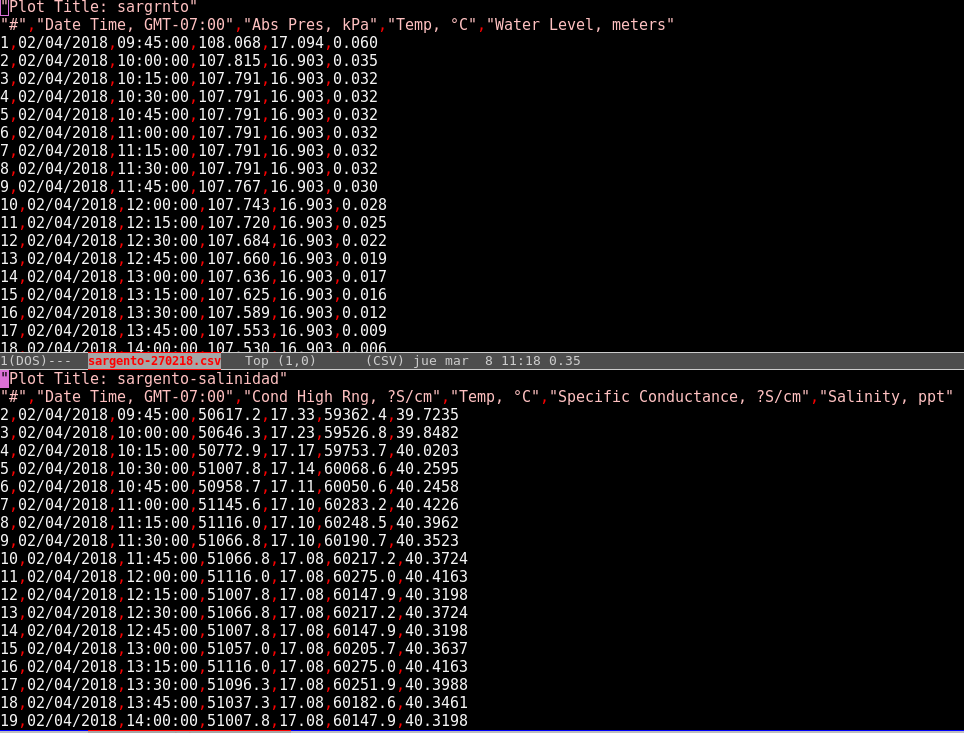
\includegraphics[width=8cm, height=8cm]{archivo.png}
\end{center}

Ya con los dos iguales, se prosigue a su posterior análisis con python, donde se crearán distintas gráficas con variadas bibliotecas.

Lo primero que se tiene que realizar en jupyter notebook es la importación de las bibliotecas a utilizar

\begin{center}
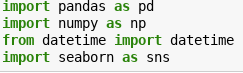
\includegraphics[width=4cm, height=2cm]{inicio.png}
\end{center}

Lo siguiente, es leer los dos archivos en cuestión. Cada uno tendrá la misma cantidad de lineas para su análisis. En esta parte se cuidará de escribir todo lo correspondiente al archivo tal cual es, si tiene coma en sus separaciones, entonces se tiene que escribir en el código. También el número de lineas que va a dejar pasar para empezar a leer el archiv0:

\begin{verbatim}

df1= pd.read_csv('sargento-270218.csv', header=None, skiprows=2, sep=',')
df2= pd.read_csv('sargento-salinidad-270218.csv', header=None, skiprows=2, sep=',')

\end{verbatim}



Cada uno de los datos contenidos en los archivos se distinguirá por df1 y df2. Cada uno tiene columnas de datos diferentes, el primero 5 y el otro 6. Se le asignará el nombre apropiado para su posterior uso.

\begin{verbatim}
df1.columns = ['#','Date','abs','temp','Met']
df2.columns = ['#','Date','CondH','temp','Conduc','sal']
\end{verbatim}

Se verificará que los datos hayan sido leídos correctamente:

\begin{verbatim}
df1.head()
df2.head()
\end{verbatim}

Que desplegará cinco líneas de datos de cada archivo en cuestión.

Lo siguiente es convertir la fecha de cada archivo en una variable temporal para la posterior utilización de ella en las gráficas a continuación.

\begin{verbatim}
df1['Ndate'] = pd.to_datetime(df1['Date'], format='%m/%d/%Y %H:%M:%S')
df1['month'] = df1['Ndate'].dt.month
\end{verbatim}

\section{Resultados-Gráficas}

Lo siguiente en la actividad es la realización de gráficas. Lo primero que se pide es la realización de tres por medio de boxplot.

La primera es de la altura del agua con respecto al tiempo que pasa. Para ello se utilizaron las bibliotecas seaborn y matplotlib.

\begin{verbatim}
import seaborn as sns
import matplotlib.pyplot as plt
ax = sns.boxplot(x="month", y="Met", data=df1)
plt.show()
\end{verbatim}

Que desplegará la gráfica a continuación:

\begin{center}

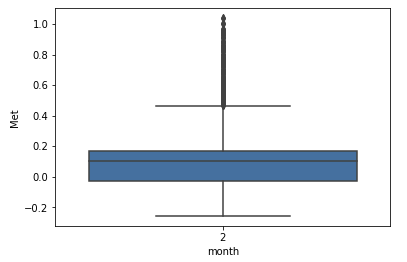
\includegraphics[width=5cm, height=5cm]{box1.png}

\end{center}

Que es la equivalente a la gráfica de altura del mar respecto al mes. Se pueden apreciar distintas cosas de la gráfica.

La gráfica y código de salinalidad respecto al mes se muestra:
\begin{verbatim}
import seaborn as sns
import matplotlib.pyplot as plt
ax = sns.boxplot(x="month", y="sal", data=df2)
plt.show()
\end{verbatim}

\begin{center}

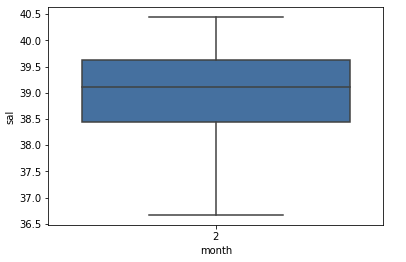
\includegraphics[width=5cm, height=5cm]{box2.png}

\end{center}

Para finalizar con la temperatura respecto al tiempo

\begin{verbatim}
import seaborn as sns
import matplotlib.pyplot as plt
ax = sns.boxplot(x="month", y="temp", data=df2)
plt.show()
\end{verbatim}

\begin{center}

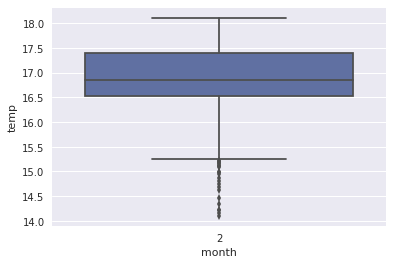
\includegraphics[width=5cm, height=5cm]{box3.png}

\end{center}

Con estas gráficas se pueden observar varias particularidades de la meteorología respecto al mes que ocurre.

Lo siguiente es usar la biblioteca seaborn, la cual nos servirá para realiazr las gráficas. Cada una tendrá la dispersión de valores más un ajuste lineal para los datos.

La primera se trata de realizar una gráfica de la altura del agua respecto a la salinalidad del agua. Arriba se muestran la comparación de la altura respecto al mes y, a la derecha, de la salinalidad respecto al tiempo. Estas presentan un ajuste lineal que mejor se ajusta a la dispersión de los datos.
\begin{verbatim}

import seaborn as sns
sns.set(style="darkgrid", color_codes=True)

g = sns.jointplot("CondH", "sal", data=df2, kind="reg",
                   color="r", size=7)
plt.show(g)

\end{verbatim}


\begin{center}

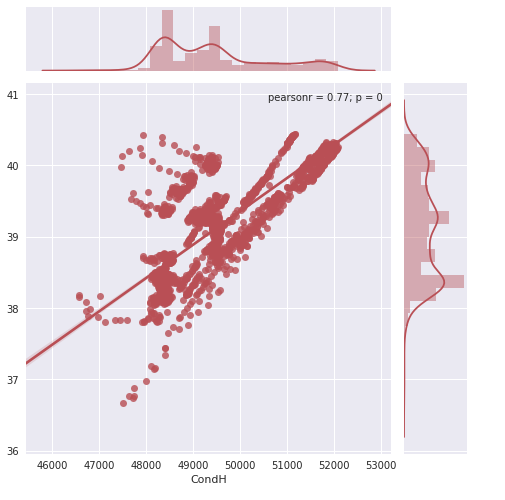
\includegraphics[width=8cm, height=8cm]{lin1.png}

\end{center}

En esta se tiene algo similar que la anterior, sólo que las variables se cambian. Se permutan la salinalidad con la temperatura
\begin{verbatim}

import seaborn as sns
sns.set(style="darkgrid", color_codes=True)

g = sns.jointplot("CondH", "temp", data=df2, kind="reg",
                   color="r", size=7)
plt.show(g)

\end{verbatim}

\begin{center}

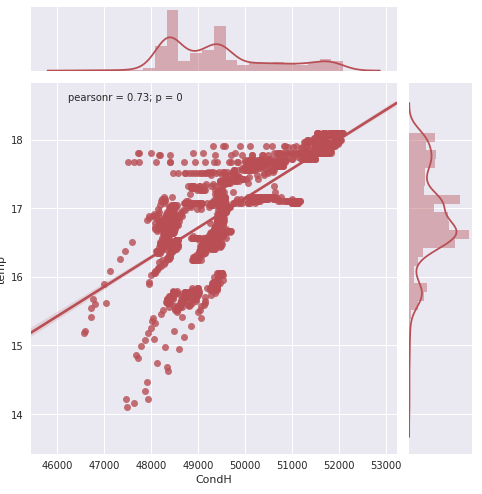
\includegraphics[width=8cm, height=8cm]{lin2.png}
\end{center}

En esta última, se utiliza la sanilalidad y la temperatura como variables a graficar.

\begin{verbatim}

import seaborn as sns
sns.set(style="darkgrid", color_codes=True)

g = sns.jointplot("sal", "temp", data=df2, kind="reg",
                   color="r", size=7)
plt.show(g)

\end{verbatim}

\begin{center}

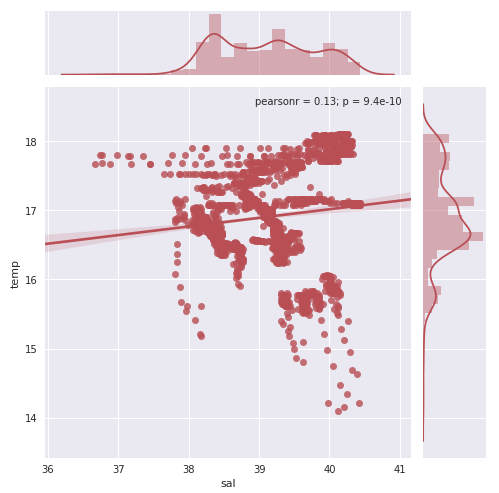
\includegraphics[width=8cm, height=8cm]{lin3.png}
\end{center}


Lo siguiente en la actividad es realizar una gráfica para distintas variables del archivo sanilidad, en éstas se tiene una comparación directa contra el tiempo.
En la primera se realizó una gráfica de la altura del agua respecto al tiempo.

\begin{verbatim}

plt.figure(); df2.CondH.plot(); plt.legend(loc='best')
plt.title("")
plt.ylabel("Tiempo")
plt.grid(True)
plt.show()

\end{verbatim}



\begin{center}
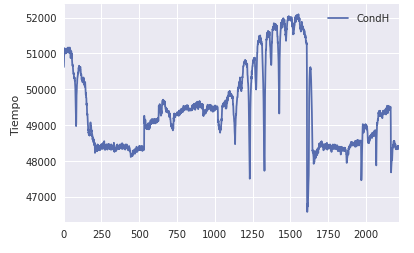
\includegraphics[width=8cm, height=8cm]{graf1.png}
\end{center}

En la siguiente se realizó una de la sanilalidad respecto al tiempo
\begin{verbatim}

plt.figure(); df2.sal.plot(); plt.legend(loc='best')
plt.title("")
plt.ylabel("Tiempo")
plt.grid(True)
plt.show()

\end{verbatim}

\begin{center}

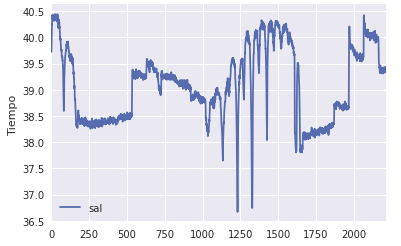
\includegraphics[width=8cm, height=8cm]{graf2.png}
\end{center}

Y por último, una de la temperatura respecto al tiempo

\begin{verbatim}
plt.figure(); df2.temp.plot(); plt.legend(loc='best')
plt.title("")
plt.ylabel("Tiempo")
plt.grid(True)
plt.show()
\end{verbatim}

\begin{center}

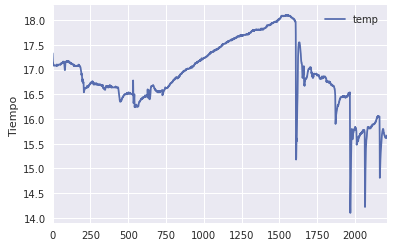
\includegraphics[width=8cm, height=8cm]{graf3.png}
\end{center}

En las gráficas anteriores se puede observar que tienen un comportamiento un poco errático, pero que casi tienen la misma forma y los picos abruptos que hacen presencia en ellos.

La penúltima actividad trata de obtener dos gráficas y superponerlas para ver las discrepancias directas que hay entre ellas.

La primera es sobre la altura del agua y sanilalidad, cómo influye el tiempo en ellas


\begin{verbatim}

plt.plot_date(x=df2.Ndate, y=df2.CondH, fmt="b-")
plt.plot_date(x=df2.Ndate, y=df2.sal, fmt="r-")
plt.title("")
plt.ylabel("")
plt.grid(True)
plt.show()

\end{verbatim}

o puede ser de la siguiente forma:

\begin{verbatim}
fig, ax1 = plt.subplots()
a=df1.HIGHT
b=df2.Date
ax1.plot(t,a, 'b-')
axa1.set_xlabel('time (s)')

ax2 = ax1. twinx()
ax2.plot(t,b, 'r.')
ax2.set_ylabel('nivel del may salinidad', color='r')
fig.tight_layout()

plt.show
\end{verbatim}


\begin{center}

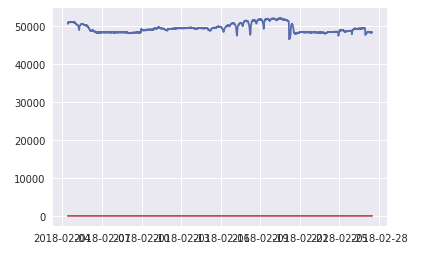
\includegraphics[width=8cm, height=8cm]{dos1.png}
\end{center}

Ésta es sobre la altura y la temperatura respecto al tiempo

\begin{verbatim}

plt.plot_date(x=df2.Ndate, y=df2.CondH, fmt="b-")
plt.plot_date(x=df2.Ndate, y=df2.temp, fmt="r-")
plt.title("")
plt.ylabel("")
plt.grid(True)
plt.show()

\end{verbatim}

O puede ser

\begin{verbatim}
fig, ax1 = plt.subplots()
a=df1.HIGHT
b=df2.temp
ax1.plot(t,a, 'b-')
axa1.set_xlabel('time (s)')

ax2 = ax1. twinx()
ax2.plot(t,b, 'r.')
ax2.set_ylabel('nivel del mar y temperatura', color='r')
fig.tight_layout()

plt.show
\end{verbatim}



\begin{center}

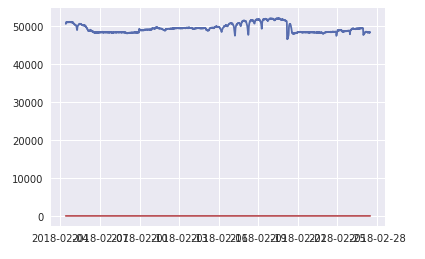
\includegraphics[width=8cm, height=8cm]{dos2.png}

\end{center}
En las gráficas anteiriores no se pueden ver muchas dicrepancias, para ello se usará un operador a continuación.

Al final, se quiere aplicar el xlim para poder ver si hay diferencias entre las dos gráficas anteriores, debido a que su espaciamiento es muy grande y casi no se puede distinguir entre ellos. Para ello se usa el comando xlim más el límite deseado para poder observar la discrepancia entre ellos.

\begin{verbatim}

df01=plt.plot_date(x=df2.Ndate, y=df2.CondH, fmt="b-")
df02=plt.plot_date(x=df2.Ndate, y=df2.temp, fmt="r-")
plt.title("")

plt.xlim([1000,1500])

plt.ylabel("")
plt.grid(True)
plt.show()

\end{verbatim}
\\
\\
\\


\begin{verbatim}
plt.plot_date(x=df2.Ndate, y=df2.CondH, fmt="b-")
plt.plot_date(x=df2.Ndate, y=df2.temp, fmt="r-")

plt.xlim([1000,1500])

plt.title("")
plt.ylabel("")
plt.grid(True)
plt.show()
\end{verbatim}

Esta instrucción hace más chica la imagen para poder enfocarnos en una parte más específica de la gráfica.

Se puede apreciar que hay una diferencia notable entre las dos gráficas que no es muy apreciable si se le ve de más "lejos".



\end{document}
